\documentclass[tikz]{standalone}
\usetikzlibrary{automata, positioning, arrows.meta}
% The automata library and loops (M5 step 4, D95): states with their default
% size and with "every state" changed, "initial" on each side with its text,
% "accepting" (double, with its outer sep), and loops on all four sides with
% their labels, next to a bend on a state.
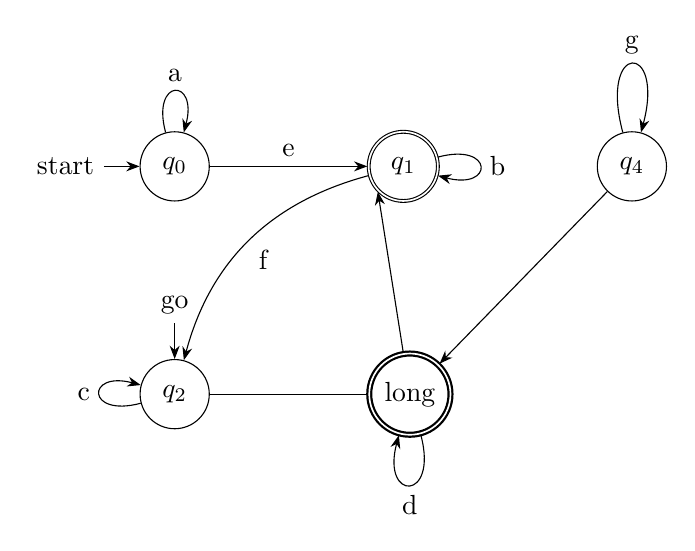
\begin{tikzpicture}[node distance=20mm, auto, >=Stealth]
  \node[state, initial]                       (q0) {$q_0$};
  \node[state, accepting, right=of q0]        (q1) {$q_1$};
  \node[state, initial above, initial text=go, below=of q0] (q2) {$q_2$};
  \node[state, accepting, thick, right=of q2] (q3) {long};
  \draw[->] (q0) to[loop above] node[name=l1] {a} (q0);
  \draw[->] (q1) to[loop right] node[name=l2] {b} (q1);
  \draw[->] (q2) to[loop left]  node[name=l3] {c} (q2);
  \draw[->] (q3) to[loop below] node[name=l4] {d} (q3);
  \draw[->] (q0) -- node[name=l5] {e} (q1);
  \draw[->] (q1) to[bend right] node[name=l6] {f} (q2);
  \draw[->] (q3) -- (q1.south west);
  \draw (q2) -- (q3.west);
  % "loop" itself sets the distances; "every loop" does too, after them.
  \node[state, right=of q1] (q4) {$q_4$};
  \path[->, every loop/.style={min distance=12mm}] (q4) edge[loop above] node[name=l7] {g} ();
  % Edges into an accepting state stop at its outer line.
  \draw[->] (q4) -- (q3);
\end{tikzpicture}
\end{document}
